\subsection{Estado inicial}
La aplicación desarrollada por Joel García y la presentada en este trabajo difieren en la manera de interactuar con el modelo. La aproximación que tomó Joel García fue la de realizar una ejecución de tres fases distintas, interactuando varias veces con el modelo. En el diagrama de la figura \ref{fig:diagrama_joel}, obtenido del trabajo de Joel García~\cite{jiragpt}, muestra el flujo de trabajo de la aplicación JiraGPT Next en su estado inicial.

\begin{figure}[H]
    \centering
    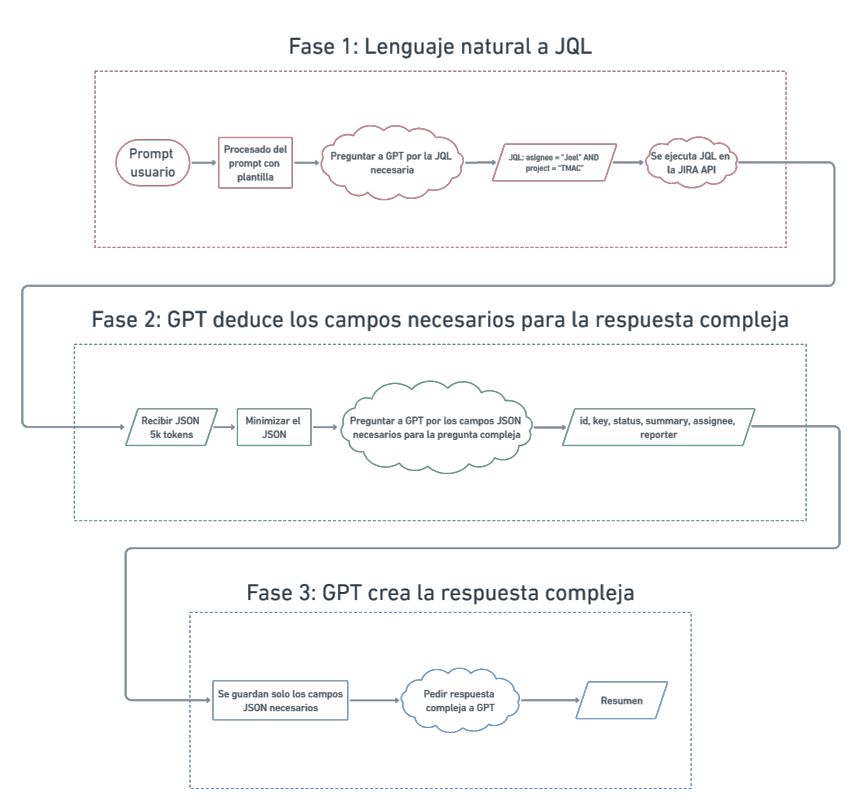
\includegraphics[width=0.95\textwidth]{images/diagrama_joel.png}
    \caption{Diagrama de las tres fases de la aplicación JiraGPT Next en su estado inicial~\cite{jiragpt}.}\label{fig:diagrama_joel}
\end{figure}

Durante la primera fase se preprocesaba la pregunta para adaptarla con plantillas y otorgar algo de contexto e indicaciones al modelo, se enviaba la pregunta y se postprocesaba la respuesta para limpiar cualquier tipo de comentario adicional que imposibilitase la ejecución de la consulta JQL. Durante esta misma fase se realizaba la llamada a la API de Jira con la consulta JQL generada ya procesada y se recogía el JSON devuelto.

La segunda fase consistía en limpiar el JSON para reducir campos de la respuesta que no contienen información relevante. En caso de no haber activado el botón de pregunta compleja, el resultado sería el JSON limpio, que se expone en la interfaz al usuario. En caso de haber activado la pregunta compleja, se haría una segunda llamada al modelo para que decidiese cuáles de los campos del JSON que se han conservado son relevantes para responder a la pregunta.

La tercera fase, que se ejecutaba independientemente de si la pregunta compleja ha sido activada, consistía en una tercera llamada para que realizase un resumen de lo preguntado. De esta manera, el usuario recibía tanto los campos que había solicitado como un resumen que respondiese a su pregunta de manera más directa.

Este proceso utilizaba la libería de Python que ofrece OpenAI para comunicarse con el modelo, de manera que resulta necesario adaptar el código para que funcione con esta librería. Lo que se propone desde este trabajo, también es una mejora en la interacción con el modelo, ya que se va a utilizar Langchain, una librería que permite la abstracción del uso del modelo, por lo que es más sencillo realizar llamadas a cualquier modelo de nuestra elección, sin tener que depender de las librerías de cada uno de los proveedores de estos modelos.

\subsubsection{Precisión inicial}
Para evaluar el estado inicial del modelo se ha de poner en contexto la técnica utilizada para evaluar la precisión: un \textit{benchmark} de 70 preguntas en el que se relaciona cada una con las incidencias que deberían ser recuperadas por el modelo.

La manera en la que se evalúa es ejecutando el conjunto entero de preguntas y comprobando si el asistente ha recuperado exactamente las incidencias contenidas en el conjunto de datos. Esto se decidió de esta manera ya que puede darse el caso en el que diferentes consultas devuelvan las mismas incidencias, lo que se consideraría correcto, con tal de que esas incidencias respondan a la pregunta del usuario.

En el momento de inicio de este trabajo, el asistente JiraGPT Next oscilaba entre un 45 y un 50\% de precisión en la recuperación de incidencias. Este resultado es fruto de una investigación sobre \textit{prompt engineering} realizada previamente por Joel García~\cite{jiragpt}. El objetivo, entonces, es buscar nuevas maneras de mejorar la precisión ofrecida por el modelo.